\chapter{Analysis}
\label{chap:analysis}
	As with so many projects, toy never start from scratch. In this chapter I will investigate exising solutions solving the same problem -- or one fairly similar to -- as desribed in chapter \ref{chap:intro}.

	\section{Existing Available Tools}
		Having reseached which tools are currently available, I've condensed my findings into the following list. 

		\begin{itemize}
			\item LastPass, and Similar Solutions
			\item KeePass, and Similar Solutions
			\item Rattic (https://rattic.org)
			\item Encryptr (https://encryptr.org/)
			\item VAULT (https://vaultproject.io/)
			\item Vault (https://www.zoho.com/vault/application-security.html)
			\item TeamPasswordManager (http://teampasswordmanager.com)
			\item Secret Server Express (http://thycotic.com/products/secret-server/express/)
			\item Simple Safe (https://www.simplesafe.net/)
			\item PassWork (https://passwork.me/)
			\item SimpleVault (http://simplevault.sourceforge.net)
			\item PasswordState (http://www.clickstudios.com.au/)
		\end{itemize}

		\subsection{LastPass, and Similar Solutions}
		\label{subsec:lastpass}
			In the name of usability services such as LastPass\footnote{https://lastpass.com/}, PassPack\footnote{https://www.passpack.com/}, DashLane\footnote{https://www.dashlane.com/}, and so many others grew popular, and it is easy to understand why. Enabling you to access your passwords from several devices, through native apps or the browser, it seemed like it was the perfect match of usability and security. To not repeat myself over and over again, I will focus on LastPass \emph{(due to them being the most well-known)} as a representation of this group.

			If we start by looking at the technical details of LastPass, they quote themselves using 256-bit AES encryption, and applies PBKDF2, in order to make it as difficult as possible, to crack stored data. For maximum security, both encryption and decryption, is done client side\cite{lastpass_cleintsideencryption}, as to avoid transferring the actual password, unencrypted, to their servers. Encryption and decryption is done using the master password, which is never actually sent to their servers. Finally, as is to be expected, all connections to LastPass' servers, are SSL encrypted.

			Having examined the technical aspect, we need to pay attention to the usability as well. Looking at their web UI, it shows a reasonably straight forward design. Allowing the user to organise passwords folders, creating a two-level structure, as seen on figure \ref{fig:lastpass_main} on page \pageref{fig:lastpass_main}. While this \emph{does} allow the user some level of organisation, several levels would have been preferable. Additionally, LastPass is renowned for their apps and plugins, covering all major operating systems and browsers, creating a near seamless integration, when it comes to addition of new passwords and auto-filling stored passwords.

			However, with the recent leak from LastPass \cite{lastpass_leak}, more and more users grew suspicious of these services. No matter how much encryption you apply, you can not get around the fact, that you have to \emph{trust} LastPass to both be completely honest about their encryption technology, \emph{and} storing your sensitive data. In many of the more sceptical user's eyes, this is a huge drawback, and why this solution is deemed unusable to solve the problem at hand.

			\begin{figure}[h!]
				\centering
				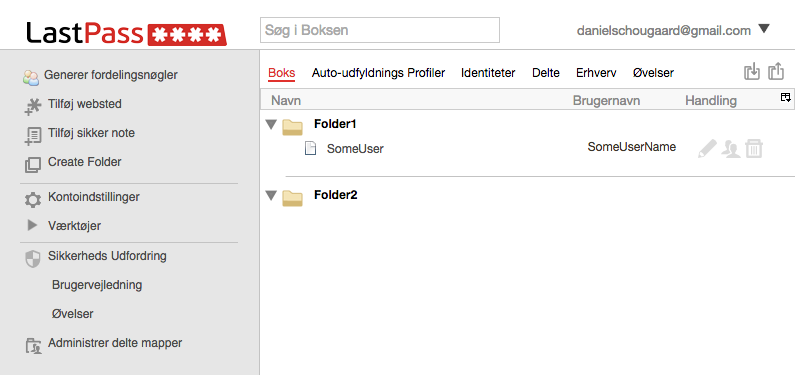
\includegraphics[width=\textwidth]{figures/analysis/lastpass_main.png}
				\caption{Screenshot of LastPass' main view, in a browser.}
				\label{fig:lastpass_main}
			\end{figure}



		\subsection{KeePass}
			As the users grew suspicious of LastPass and the likes, a lot of them moved over to e.g. KeePass\footnote{https://keepass.org}. While there exists a plethora of tools similar to KeePass, I will focus on KeePass as the representative of the bunch, much as in section \ref{subsec:lastpass}.

			If we again start by examining the technical details, as of version 2.x KeePass only -- per default -- offers AES-256 encryption, which is seen on figure \ref{fig:keepass_create_security} on page \pageref{fig:keepass_create_security}, with additional algorithm choices available through plugins \cite{keepass_security}. This enables users to tailor the encryption security, to their own needs -- and beliefs. 

			Looking at the main UI, of which an example is shown on figure \ref{fig:keepass_main} on page \pageref{fig:keepass_main}, KeePass features exactly that which could be improved in LastPass: A tree like structure, in order to completely organise passwords. Other than that, there isn't anything noteworty to say about their UI: It features the necessary and that's about it. A final thing worth mentioning, is that their password generator is completely customisable, as seen on figure \ref{fig:keepass_newpassword_passwordgen} on page \pageref{fig:keepass_newpassword_passwordgen}. You can manually choose, exactly which character sets, you wish to be in your passwords, enabling you to have passwords using local accents should the target system support it, which is a really nifty feature.




			\begin{figure}[h!]
				\centering
				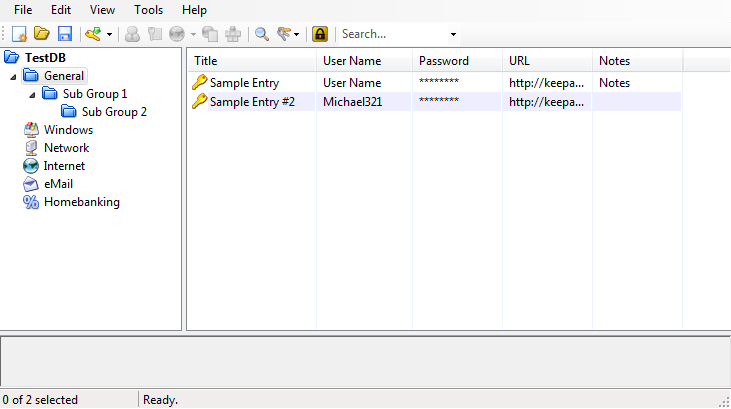
\includegraphics[width=\textwidth]{figures/analysis/keepass_mainview.png}
				\caption{Screenshot of KeePass' main view.}
				\label{fig:keepass_main}
			\end{figure}

			\begin{figure}[h!]
				\centering
				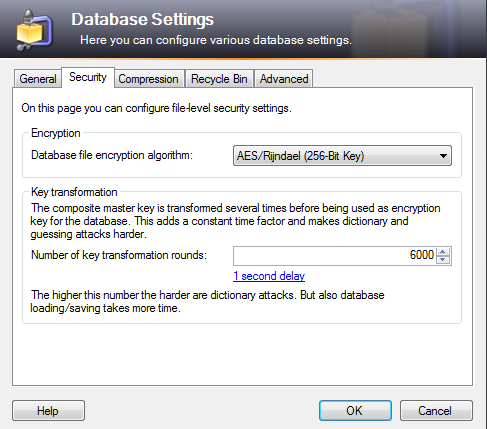
\includegraphics[width=0.7\textwidth]{figures/analysis/keepass_create_security.png}
				\caption{Screenshot of KeePass' security options.}
				\label{fig:keepass_create_security}
			\end{figure}
		
			%\begin{figure}[h!]
			%	\centering
			%	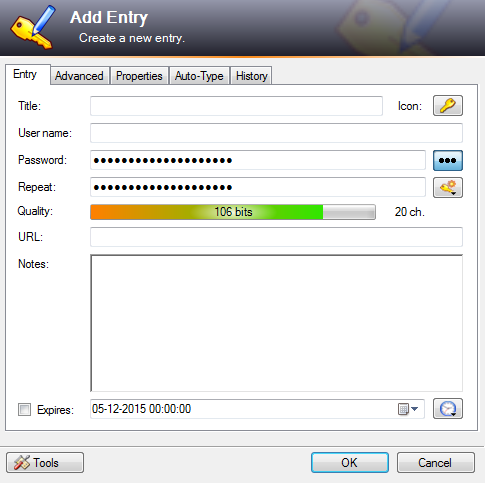
\includegraphics[width=\textwidth]{figures/analysis/keepass_newpassword_main.png}
			%	\caption{.}
			%	\label{fig:}
			%\end{figure}

			\begin{figure}[h!]
				\centering
				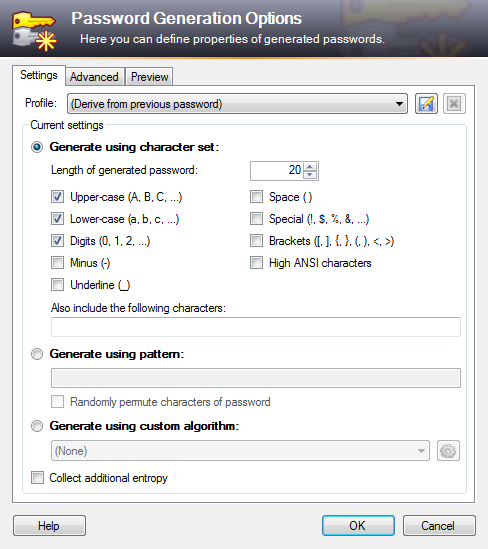
\includegraphics[width=0.7\textwidth]{figures/analysis/keepass_newpassword_passwordgen.png}
				\caption{Screenshot of KeePass' password generator settings.}
				\label{fig:keepass_newpassword_passwordgen}
			\end{figure}







		\subsection{KeePass \& Other Locally Stored Password Managers}
			Since the breach of LastPass, KeePass and the like have been the go-to tools, for storing, generating and retrieving passwords. While most of these tools are very user-friendly, very intuitive, and very secure, they do lack one very important aspect: Accessibility. All of these tools store the passwords, in an encrypted file on the disk of the local machine.

			While there exists a plethora of similar solutions, I will focus on KeePass for this section.P

			KeePass' organisational options are brilliant. Its tree structure, enables you to easily organise your passwords.While one could argue, that this is "enough", we also have to face that we live in the age of electronics. Almost everybody has at least \emph{two} devices, both of which would need access to passwords. Hence, KeePass and the like suffer from the fact, that you would need a 3rd party way to distribute these files. One option to this is Dropbox. But again: This just destroys the user-friendliness of the workflow.

			KeePass uses AES-256, compressed with GZIp


		\subsection{Rattic}
			Rattic is almost what a good password manager should be: Simple, lightweight, and easy to use. That is, except that it is obviously aimed at teams. The most apparent indicator of this, is the fact that a newly created password needs to be assigned to a "Group". This would be fine, had Rattic taken a hint from Unix, creating a personal group for each user. But alas, no. You'd need to manually create a new group, for each user, to be able to store private passwords in Rattic.

			Additionally, Rattic suffers from lack of a tree stucture. You have \emph{two} options of sorting passwords: Groups and tags. Neither of which is presented in a manner, that gives a quick overview of the contents of the databse, or allows for more than a single level of hierarchy. Supports export in KeePass format.
			
			While this software could essentially suffice, in order to meet the requirements, it would be lacking heavily in the user experience department.


		\subsection{Encryptr}
			Encryptr is a very interesting piece of software. Developed by SpiderOak, it offers zero-knowledge encrypted password storage, using the Crypton backend. However, per default it uses SpiderOaks servers, running Crypton. This puts Encryptr basically in the same overall category as LastPass: You need to trust someone else with your sensitive information. 

			Luckily, you \emph{can} run the Crypton backend at home. Unfortunately, getting this Crypton to work is not as straight forward as one could've hoped. Ontop of that, getting Encryptr to work with your own Crypton server, requires editing code, to change the target server. Hence, for this purpose Encryptr is \emph{very} bad, when it comes to usability.

		\subsection{Vault}
			ZOHO's Vault software is yet another piece of software that falls under the same category as LastPass: You upload your passwords to their servers. While they -- much like LastPass -- have a delightful UI and good user experience, it is \emph{still} hosted on a machine, someone else hosts.

			
		\subsection{VAULT (vaultproject.io)}
			Vault markets itself as a tool for ``securely accessing secrets". This tool differs greatly from the previously covered. Vault is \emph{only} a CLI / HTTP API tool. There is no graphical interface as such.

		\subsection{TeamPasswordManager}
			TeamPasswordManager aims itself at -- as the name implies -- teams, much like Rattic. This choice, is very apparent in the work flow. For instance, a password is tied to a ``project", instead of a user. Security wise, TeamPasswordManager dons some impressive features. Using the standard AES-256, with the twist of a Bcrypt approach, and two-factor authentication.

			While this software could essentially suffice, in order to meet the requirements, it would be lacking heavily in the user experience department.



		\subsection{Secret Server Express}
			Thycotic's Secret Server Express is yet another one of those pieces of software, clearly aimed at the Enterprise. Their feature list is surely impressive, but most of them are clearly aimed at larger corporations. 

			Giving no demo or screenshots of the software they're selling, it is impossible to determine the user experience of the software, however I would go as far as to wager, that it would be very focussed on enterprise workflows.

		\subsection{Simple Safe}
			Simple Safe markets itself at teams, which is not necessarily evident at a first glance. However, based on their own user experience -- and poor description -- it appears that all users have access to all passwords. This results in, that a single user can not have a private password, for their use only.

			As seen before, Simple Safe allows passwords to be organised in "groups", much like Rattic. When you switch between groups, it is very ``clonky", with a grey'ed over screen, showing it's loading -- and it takes a while. From a user experience point of view, their solution is less than optimal.

			From a encryption perspective, there isn't a lot to be told. Their rather vague description of their software, only states that they use 256 bit encryption \footnote{https://www.simplesafe.net/faqs/}, omitting their algorithm choice.


		\subsection{PassWork}
			Yet another solution, that markets itself at the enterprise, and has password data stored on a remote server. Same comments goes for this, as for LastPass, Vault (ZOHO), and Secret Server Express. 

			Their user experience seems fine, and at first glance they -- per default -- have created a private group for each user, to store private passwords in. 

		\subsection{Simple Vault}
			While Simple Vault is \emph{clearly} not aimed at enterprise use and is actually self-hosted, it does come with a bunch of downsides. First of all, it does not appear that it has the possibility for several users. Secondly, there is absolutely \emph{no} organisation: Passwords are stored single level, sorted lexicographical. Each individual password, can be protected by a passphrase, ``sort of" enabling multi-user access. However, other users will be able to see the password exists for a given website, which can be considered unfortunate.

			User experience wise, it is horrible. The design and colours are a pain to work with, the position of buttons and menus are not intuitive. Not to sound too harsh, but the design looks like it was made by a 7th grader: It does \emph{not} inspire confidence, in the developers ability to sufficiently protect my data.s

		\subsection{PasswordState}
			While PasswordState does market itself at enterprise customers, they offer a free version of their software, for teams of up to five people. Their UI is wonderful, if you are a tech geek and/or love graphs. It is very advanced since you're immediately presented with a lot of information, leading to believe it would easy scare off not-so-super-users.

			Sporting a tree level structure, PasswordState manages to create the organisation there have been lacking from the previously examined tools.

			Unfortunately, PasswordState is limited to the Windows platform, making it less than optimal for the purposes of this project. It would render it unable to be executed, from a Raspberry Pi, for instance.







	\section{Academic Research and Tools}
	\section{Chosen Inspiration}